\documentclass{beamer}


\usepackage{listings}
\lstloadlanguages{python}


\usepackage{tikz}
\mode<presentation>
{
\usetheme{Singapore}
  \setbeamercovered{transparent}
   \setbeamertemplate{footline}[frame number] 
  \setbeamertemplate{navigation symbols}{ 
  \insertslidenavigationsymbol
  \insertframenavigationsymbol
  \insertsubsectionnavigationsymbol
  \insertsectionnavigationsymbol
  \insertdocnavigationsymbol
  \insertbackfindforwardnavigationsymbol
  \hskip 0.3cm
  %\insertframenumber / \inserttotalframenumber  % <<< frame #
  %\insertpagenumber / \insertpresentationendpage % <<< page #
} 
}

\usepackage[english]{babel}
\usepackage[latin1]{inputenc}
\title{ILCDIRAC}
\subtitle{A grid solution for the LC community}
\author{St\'ephane Poss et al.}
\institute[CERN]
{
 CERN
}
\date{\today}
% This is only inserted into the PDF information catalog. Can be left
% out.
\subject{ILCDIRAC}



% If you have a file called "university-logo-filename.xxx", where xxx
% is a graphic format that can be processed by latex or pdflatex,
% resp., then you can add a logo as follows:

% \pgfdeclareimage[height=0.5cm]{university-logo}{university-logo-filename}
% \logo{\pgfuseimage{university-logo}}
\AtBeginSubsection[]
{
\begin{frame}<beamer>
\frametitle{Outline}
\tableofcontents[currentsection,currentsubsection]
\end{frame}
}


\begin{document}
\begin{frame}
\titlepage
\end{frame}

\begin{frame}
  \tableofcontents
\end{frame}

\section{ILCDIRAC context}
\label{sec:context}

\begin{frame}
  \frametitle{ILC VO}
The {\color{blue} ILC VO} is dedicated to the study of \alert{future
  Linear Colliders: ILC and CLIC}, specifically the study of the
detectors' concepts: ILD and SID\\
~\\
Members of the VO in DESY (DE), KEK (JP), CERN (CH), SLAC (USA), PNNL
(USA), LAPP (FR), VINCA (R.S.), etc.
\end{frame}

\begin{frame}
  \frametitle{ILCDIRAC motivations and context}
  \begin{itemize}
  \item Need for distributed analysis framework for mass production of
    MC data
    \begin{itemize}
    \item CLIC CDR had to be written
    \item Now SID DBD is being written
    \end{itemize}
  \item Evalutation of existing solutions: DIRAC was thought to
    answer the needs
  \item Needed framework for supporting the ILC VO applications:
    generation, simulation and reconstruction for both detector concepts 
  \item File catalog: metadata and replica information.
  \end{itemize}
~\\
~\\
\hspace{4cm} \alert{ILCDIRAC was born}

\end{frame}

\section{DIRAC usage}
\begin{frame}
  \frametitle{Usage}
ILCDIRAC uses most services:
\begin{itemize}
\item Framework
\item Accounting
\item Workload management
\item Request management
\item Data management: File catalog, stager, storage element, etc.
\item Transformation system: production job management
\end{itemize}
Not using Resource Status System yet!
\end{frame}

\section{Performance}
\begin{frame}
  \frametitle{Performance achieved in 2 years}
  \begin{columns}
    \column{0.5\textwidth}
    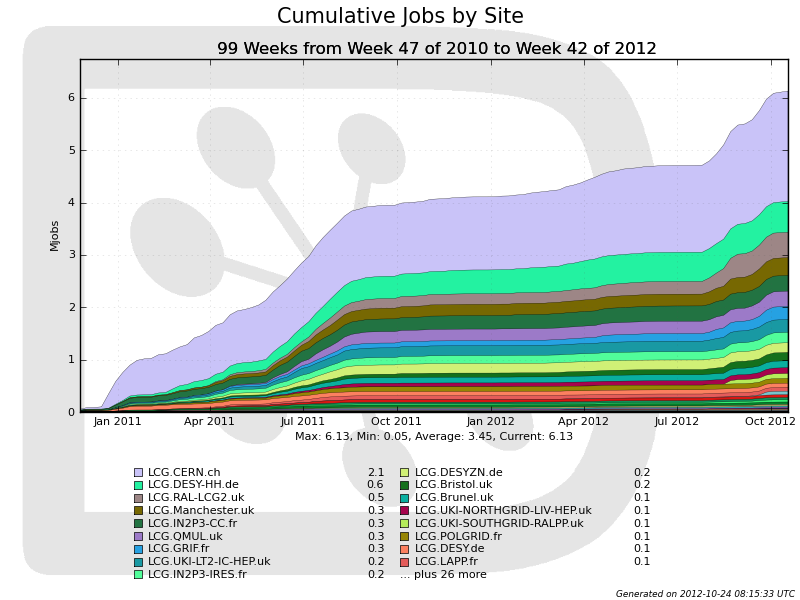
\includegraphics[width=1\textwidth]{JobsPerSite.png}\\
    Ran more than 6 million jobs in $\approx$ 50 sites
    \column{0.5\textwidth}
    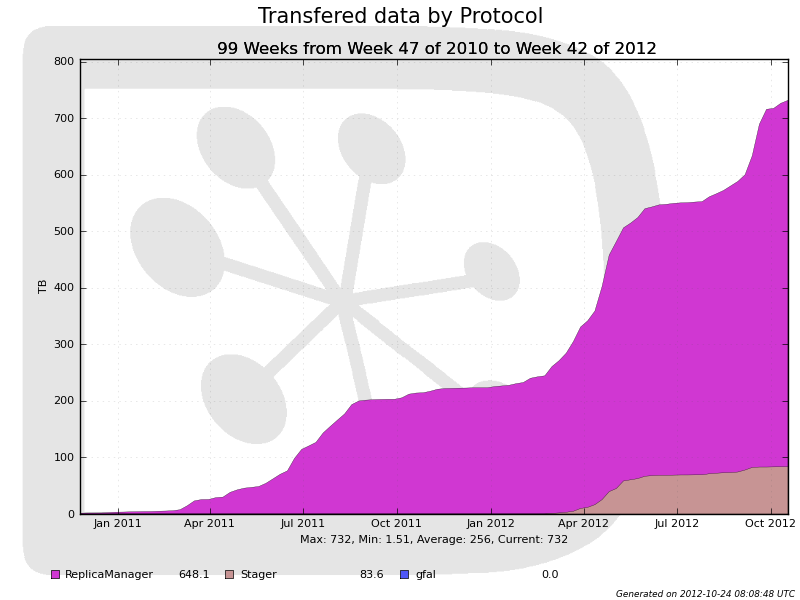
\includegraphics[width=1\textwidth]{TransferedDataPerProtocol.png}\\
    Transfered more than 730 TB between sites
  \end{columns}
~\\
~\\
6 million LFNs in the File Catalog and associated meta data.
\end{frame}

\section{Interface developments}
\label{sec:interface}
\begin{frame}
  \frametitle{Interface developments}
What we started with:
\begin{itemize}
\item Interface inspired from LHCbJob interface
\item Applications are handled in one python module, all in one class
\item No relations between them: all applications redefine everything
\item Using output of one application as input to another was cumbersome.
\item Most of all: maintenance and additions very time consuming
\end{itemize}
~\\
After 1.5 years, we needed a new interface system!
\end{frame}
\begin{frame}
  \frametitle{Redesigning the job interface}
Motivation: separate the job definition from the application
definition, add \alert{flexibility}, ease \alert{maintenance}
\begin{itemize}
\item What is an application? 
\begin{itemize}
\item Convert something into something else, or produce something out
  of nothing
\item Has a name, and certainly a version
\item Needs instructions on what to do (parameters, or set of
  parameters)
\item Produces log files
\item Can produce something that could be used by another application in
  the same job
\end{itemize}
\item What kind of jobs:
\begin{itemize}
\item User jobs: all inputs can be different for every job
\item Production jobs: all jobs share the same properties, but the
  input changes, preferably automatically (Transformation system)
\end{itemize}
\end{itemize}
\end{frame}

\begin{frame}
  \frametitle{Applications handling}
Motivation: Provide a general framework for handling any application,
using the Workflow functionality of DIRAC
\centering 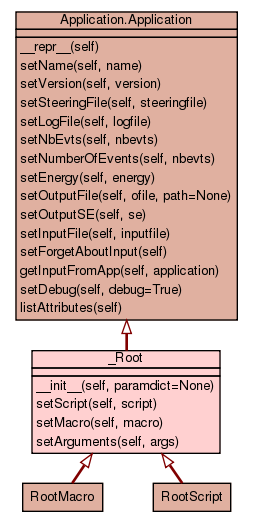
\includegraphics[width=0.25\textwidth]{ApplicationClassExample.png}\\
This example: how ROOT is handled
\end{frame}
\begin{frame}
  \frametitle{Job types}
\centering
 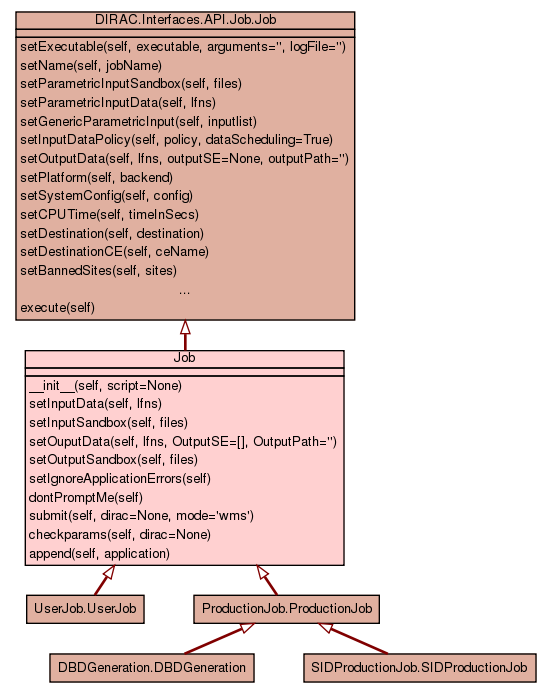
\includegraphics[width=0.5\textwidth]{JobClassDiagram.png}\\
\end{frame}
\begin{frame}
  \frametitle{Job types}
User jobs (UserJob):
\begin{itemize}
\item All jobs can have different set of inputs/parameters
\item Jobs are directly submitted to Workload Management System
\item Goes throught the Dirac API
\end{itemize}
~\\
Production jobs (ProductionJob):
\begin{itemize}
\item All jobs share the same parameters, only the input is
  different
  \begin{itemize}
  \item No local input sandbox allowed, only LFNs!
  \end{itemize}
\item Workflow is submitted to the Transformation System which creates
  the jobs on request, setting the right input (if any) 
\item Cannot go through Dirac API, but easy to create a UserJob out of it
\end{itemize}
\alert{Application definition does NOT depend on the job type.}
\end{frame}

\begin{frame}
  \frametitle{Example of a UserJob}
\lstinputlisting[language=python,basicstyle=\scriptsize]{example.py}
Check \url{http://lcd-data.web.cern.ch/lcd-data/doc/ilcdiracdoc/} for API documentation.
\end{frame}
\begin{frame}
  \frametitle{Advantages}
\begin{itemize}
\item Adding an application is independent of the job: \alert{inherit from
  the Application class} and add whatever parameter you need, also need
  to create the workflow module (I provide a base module class)
\item Adding a certain job type with different handling of (for
  example) the output is easier: \alert{inherit from the Job class} and
  implement one method. \alert{UserJob and ProductionJob} are already suitable
  for most applications
\item \alert{Maintenance} is easier
\end{itemize}
Code elements are available for anyone willing to try it. Some bits in
the DIRAC Dirac.py and Job.py class would need changes to simplify the
code.
\end{frame}

\section{Conclusion}
\label{sec:conclusion}
\begin{frame}
  \frametitle{Conclusion}
  \begin{itemize}
  \item Very successful usage of DIRAC
  \item Very successful collaboration with DIRAC developers
  \end{itemize}
~\\
Redesign of the ILCDIRAC job interface in a model that can be used by
others: code elements are available, should be imported in DIRAC for
optimal usage.\\
~\\
My contract ends at the end of this year: A.~Sailer and C.~Grefe will
take over
\end{frame}
\end{document}

% Local Variables:
% TeX-PDF-mode: t
% End:
